\documentclass[a4paper,12pt]{article}
\usepackage{caption}
\usepackage{graphicx}
\graphicspath{ {img/} }
\usepackage{fancyhdr}
\pagestyle{fancy}
\lhead{tqvj24}
\chead{}
\rhead{Image Processing Assignment}

\begin{document}

\section*{Discussion/detail of system design and choices made (5\%)}
\subsection*{System Design}
% python 3.5.2, opencv 3.1.0
% gui based, key commands, explain image layout
% modular processing, in steps, individual methods
% explain each step? With examples under 'evidence' section

\subsection*{Choices Made}
% bit shifting before converting to 8bit for more detail
% removing border via dialation (biggest contour didn't work because of clusters)
% threshold vs histogram equilisation
% comparison to ground truth (very high percentages because of big borders and empty spaces)
% detecting if dead or alive (isContourConvex was bad)

\section*{Evidence of the success of system in performing the specified task (5\%)}
\subsection*{Processing Steps}
% include images here of each step
% 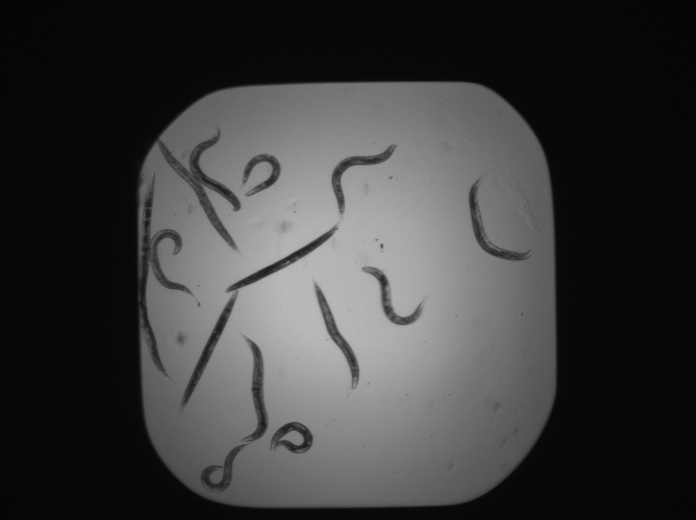
\includegraphics[width=0.95\textwidth]{A01_step0.jpg}  % for example

\centering{tqvj24}
\end{document}
